
\documentclass[11pt,a4paper]{article}

% --- Encoding and typography ---
\usepackage[T1]{fontenc}
\usepackage[utf8]{inputenc}
\usepackage{lmodern}
\usepackage{microtype}

% --- Layout ---
\usepackage[a4paper,margin=1in]{geometry}
\usepackage{setspace}
\onehalfspacing

% --- Math, tables, figures ---
\usepackage{amsmath,amssymb}
\usepackage{booktabs}
\usepackage{graphicx}
\usepackage{subcaption}
\usepackage{siunitx}
\usepackage{url}

% --- References (simple and journal-compatible baseline) ---
\usepackage[numbers,sort&compress]{natbib}

\title{Unifying Search Paradigms using optDSL}
\author{
  Michael Bögl
}
\date{\today}

\begin{document}
\maketitle

\begin{abstract}
In practical combinatorial optimization, solver-paradigm decisions are frequently made at an early project stage.
Such early commitments constrain subsequent modeling choices and can render later paradigm changes technically and organizationally costly.
This report addresses that limitation through a workflow that enables paradigm switching over the full project lifecycle.
The workflow is based on \texttt{optDSL} as a shared problem representation, leveraging its existing MiniZinc translation and extending the same representation with a Large Neighborhood Search (LNS) backend.
We detail the LNS design, including operator profiles, initialization strategies, and restart mechanisms, and evaluate the approach on benchmark instances from multiple problem classes.
Under fixed iteration and time budgets, we compare LNS-based heuristic search with a MiniZinc-based exact baseline on identical \texttt{optDSL} instances, and we further demonstrate practical applicability on a real-world use case within an extensible, model-driven optimization workflow.
\end{abstract}

\section{Introduction}
Combinatorial optimization practitioners routinely face a tension between solution quality, computation time, and implementation effort.
In many real projects, model requirements evolve over time, while the decision for a solver paradigm is made early and is difficult to revise later.
This creates a methodological lock-in that reduces both technical flexibility and practical efficiency.

Exact methods provide strong guarantees, most notably provable optimality and bounds on solution quality.
These properties are essential when results must be validated formally.
However, exact methods also exhibit well-known drawbacks.
Their computational cost can grow prohibitively on large or highly constrained instances, so that no acceptable solution may be available within practical time limits.
Their performance is sensitive to formulation quality, solver configuration, and available hardware, which makes results difficult to predict in advance.
Moreover, tight integration with a specific solver technology increases the engineering cost of model changes and rapid iteration.

Heuristic and metaheuristic methods occupy the opposite end of this trade-off.
They typically deliver good solutions quickly, scale to large instances, and can exploit domain structure through tailored search strategies.
This makes them attractive under strict runtime limits or in settings with frequent re-optimization.
Their drawbacks mirror their strengths: they provide no global optimality guarantees and usually no quality bounds, so the gap to the optimum remains unknown.
Their performance depends strongly on design choices such as operators, initialization, restart policies, and parameter settings, and a configuration that works well for one problem class may transfer poorly to another.
Consequently, substantial development and tuning effort is often required before a heuristic becomes reliable in practice.

Neither paradigm dominates the other; their strengths and weaknesses are largely complementary.
Which paradigm is preferable typically changes over the course of a project, for example when instance sizes grow, when time budgets shrink, or when formal quality guarantees become necessary.
This observation motivates a unifying approach in which the problem is modeled once and the solution paradigm remains exchangeable.

\texttt{optDSL}, a Python-inspired domain-specific language for describing optimization problems, provides such a unifying representation.
A single \texttt{optDSL} model can be dispatched to conceptually different backends:
an exact backend, currently realized through a translation to the constraint modeling language MiniZinc and its portfolio of solvers, and
a heuristic backend, currently realized through a Large Neighborhood Search (LNS) framework that operates directly on \texttt{optDSL} decision variables.
Because both backends consume identical problem descriptions, users can defer the paradigm decision, switch paradigms as project requirements evolve, and compare both paradigms under a common protocol without re-modeling.
A single \texttt{optDSL} model is fed through an importer into two parallel pipelines, one deriving the MiniZinc representation for exact solvers and one operating directly on the \texttt{optDSL} decision variables inside the LNS framework.
Beyond this dispatch view, the architecture admits a forward-looking perspective, illustrated in Figure~\ref{fig:optdsl-validation}: a solution that the LNS backend writes back in \texttt{optDSL} format can be re-injected into the exact pipeline, where the MiniZinc representation and its solvers are used to validate and improve the solution and to derive quality bounds. This closes the loop between heuristic and formal optimization within one consistent, model-centric workflow.

\begin{figure}[t]
\centering
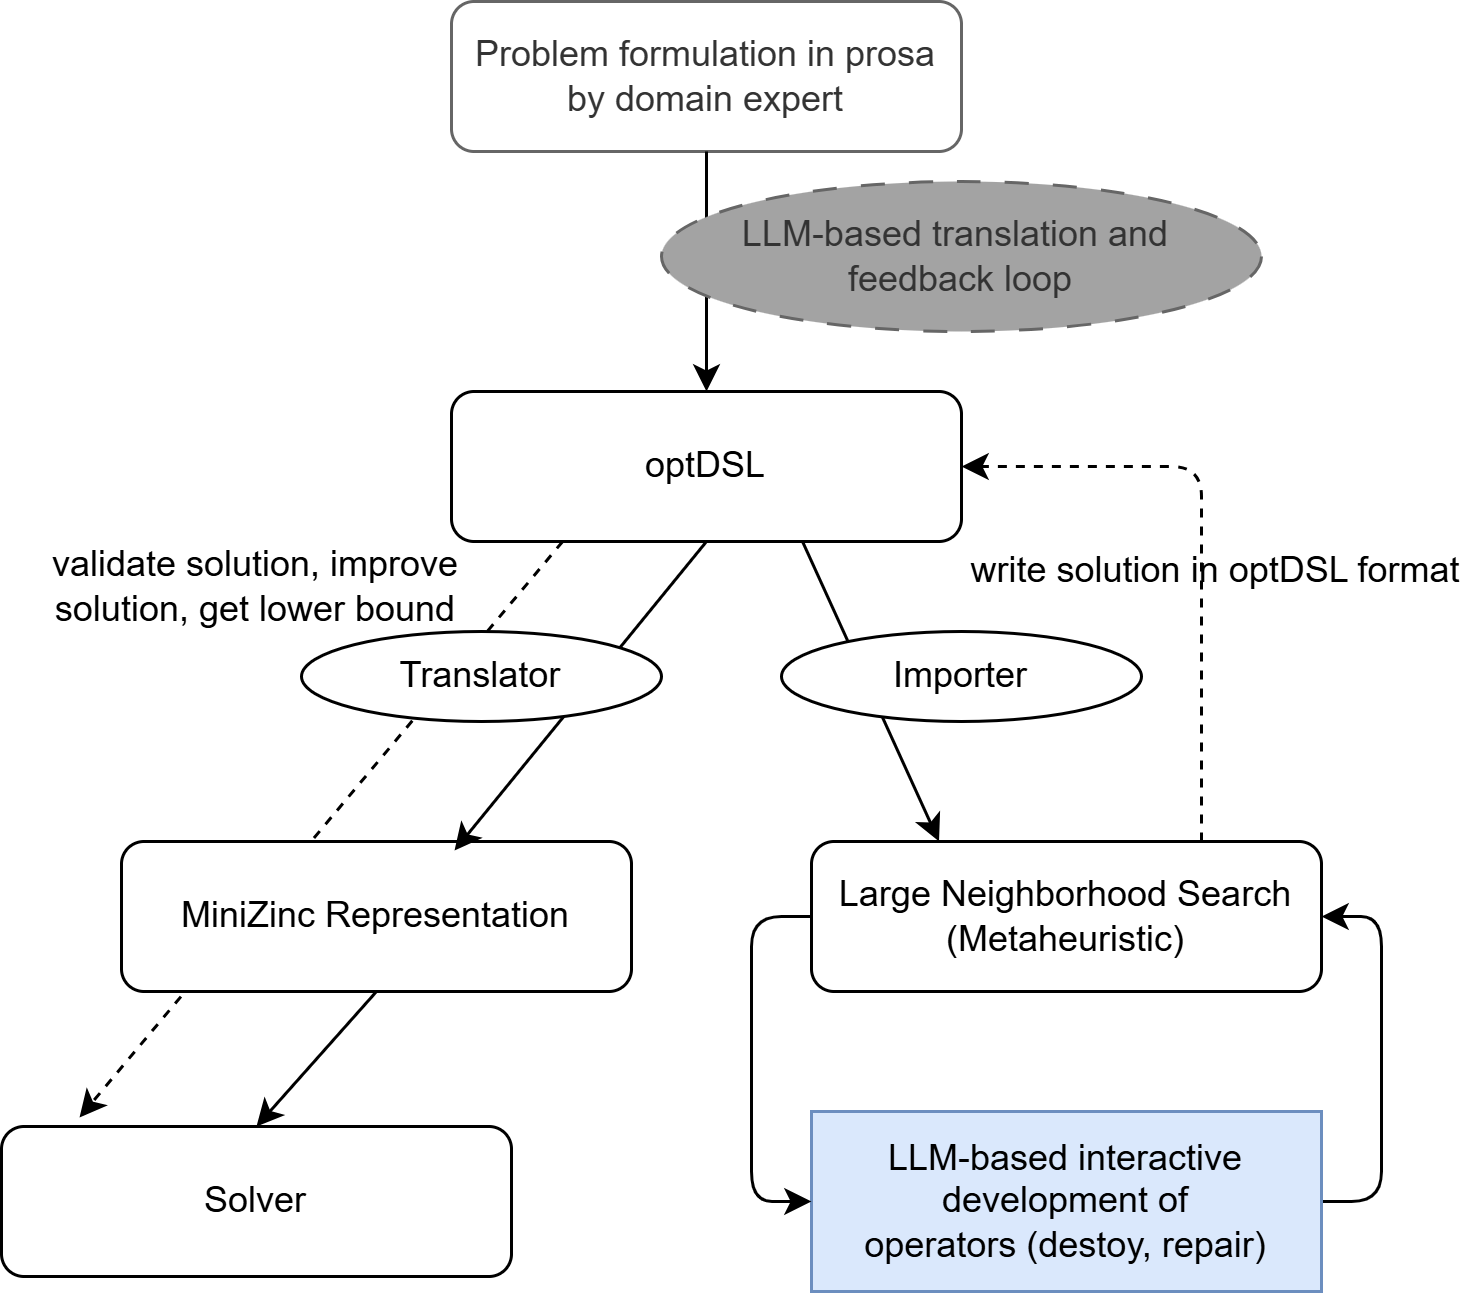
\includegraphics[width=0.6\textwidth]{optDSL_validation.drawio.png}
\caption{Perspective of the unifying workflow: a solution produced in \texttt{optDSL} format is fed back into the exact pipeline, where the MiniZinc representation and solver validate and improve the solution and provide quality bounds (e.g.\ a lower bound on the objective).}
\label{fig:optdsl-validation}
\end{figure}

This report focuses on the design and evaluation of the LNS backend within this unified architecture.

We describe the implemented operator profiles, initialization strategies, and restart mechanisms, and evaluate the resulting search behavior on benchmark instances from multiple problem classes against the MiniZinc-based exact backend on identical \texttt{optDSL} instances.
The objective is twofold: to study how far adaptive LNS design can close the quality gap under fixed compute budgets, and to demonstrate the practical value of a model-centric workflow in which the solver strategy can be revised throughout the project lifecycle.

\section{Related Work}
Research on combinatorial optimization has increasingly moved from a strict exact-versus-heuristic dichotomy toward hybrid algorithms that combine the strengths of both paradigms.
In exact optimization, rich modeling languages and solver portfolios have improved accessibility and reproducibility, with MiniZinc becoming a standard interface for expressing models independently of the backend solver \citep{nethercote2007minizinc,stuckey2014minizinc}.
In parallel, neighborhood-based metaheuristics evolved from problem-specific local search to large-scale destroy-and-repair frameworks, where very large moves can be explored while preserving feasibility through structured repair \citep{shaw1998lns,ropke2006alns,pisinger2010lns,pisinger2019lns}.

An important algorithmic line that narrows the quality-runtime gap is the use of exact neighborhoods or exact reasoning inside heuristic search loops.
In mixed-integer optimization, local branching and relaxation-induced neighborhoods are representative bridge mechanisms: they constrain search to a promising region that can still be solved (approximately or exactly) by mathematical programming machinery \citep{fischetti2003localbranching,danna2005rin}.
The same principle appears in CP-LNS workflows, where exact propagation and constraint reasoning guide neighborhood repair, while the outer search remains heuristic and anytime \citep{shaw1998lns,pisinger2010lns,pisinger2019lns}.
Conceptually, these methods trade global proof guarantees for faster high-quality improvement, but recover part of exact-method robustness through bounded or solver-driven subproblems.

For routing, this bridge perspective is particularly visible in VRP and VRPTW.
Benchmark culture and instance standardization (e.g., Solomon and later CVRPLIB developments) enabled fair comparisons between exact, heuristic, and hybrid methods under shared protocols \citep{solomon1987vrptw,toth2014vrp,uchoa2017cvrplib}.
ALNS variants in this domain demonstrate that adaptive operator selection can substantially reduce the performance gap to exact baselines on larger instances where full proofs are expensive \citep{ropke2006alns,pisinger2010lns,pisinger2019lns}.

For packing and scheduling, the same pattern recurs with different primitives.
In two-dimensional bin packing, exact bounds and formulations are often paired with constructive and improvement heuristics in matheuristic pipelines \citep{lodi2002twodimensional,hopper2001genetic,hopper2001ejor,berkey1987,wang1983}.
In job shop scheduling, classic methods such as shifting bottleneck and tabu-search-based improvements can be interpreted as structured relax-and-improve strategies that inject stronger local reasoning than pure black-box metaheuristics \citep{adams1988shifting,taillard1993benchmarks,jain1999jssp,lawrence1984,applegate1991,storer1992}.
Across these classes, the literature suggests that performance gains arise when heuristic diversification is coupled with model-aware intensification.

A prerequisite for such cross-paradigm studies is a shared problem representation that both exact and heuristic solvers can consume.
optDSL addresses this need: it is a Python-inspired domain-specific language for formulating optimization problems, and a translation from optDSL to MiniZinc has been described and published \citep{delrio2026optdsl}, enabling optDSL instances to be solved by any MiniZinc-compatible backend solver.
The present report builds directly on that work.
Rather than proposing a new modeling language or a new translation pipeline, it uses the existing optDSL representation and MiniZinc translation as a foundation and contributes an experimental study that runs LNS-based heuristic search and MiniZinc-based exact solving on the same optDSL instances.
This enables an apples-to-apples comparison of how much algorithmic gap can be closed through shared instance engineering and adaptive neighborhood design across multiple problem classes, within the bridge-algorithm tradition described above.

\section{Method}
\subsection{optDSL Representation}
All benchmark instances are provided as standalone \texttt{optDSL} models
in which data, decision variables, constraints, and the objective form a
single self-contained file.
Syntactically, an \texttt{optDSL} model is a Python-inspired DSL
\citep{delrio2026optdsl}: scalar and array data are declared as typed
constants (e.g.\ \texttt{DSList(N, DSInt())} for integer arrays), decision
variables are declared with an explicit finite domain, feasibility
constraints are written as \texttt{assert} statements over (potentially
nested) loops and arithmetic, and the objective is declared as a final
\texttt{minimize(objective)} statement.
Because both backends consume exactly this file---the exact backend through
the translation to MiniZinc \citep{delrio2026optdsl}, the LNS backend
directly on the declared decision variables---no re-modeling is required
when switching between them.
We now summarize the model structure for the three main benchmark classes;
each relies on linear arithmetic over bounded integer domains, which keeps
the MiniZinc translation straightforward.

\textbf{Two-dimensional bin packing (2DBP).}
The model operates on three finite-domain decision-variable arrays
(\texttt{assignments}, \texttt{x\_positions}, \texttt{y\_positions}):
every item $i$ is assigned to a box $b$ and placed at a lower-left corner
$(x_i,y_i)$.
Feasibility is enforced by two constraint blocks: \texttt{all\_assigned}
ensures that each item receives exactly one box, and \texttt{no\_overlap}
first requires that each item fits within the dimensions of its selected
box and then requires, for any two items in the same box, that they do not
overlap in either the horizontal or the vertical direction.
The objective counts the number of distinct boxes in use and is minimized.
The converted benchmark instances live under
\texttt{problem\_instances/2dbp/benchmarks/testset\_paper\_optdsl/} and
contain 20 items on $10 \times 10$ bins.

\textbf{Capacitated vehicle routing (CVRP).}
Two semantically equivalent encodings are used, which illustrates that
\texttt{optDSL} permits representation choices tailored to the backend.
The \emph{arc-based} encoding declares a flat binary array
\texttt{arcs[v,i,j]} (with index $v\cdot n^2 + i\cdot n + j$), a binary
\texttt{vehicle\_used} indicator, and MTZ load variables \texttt{u}.
Constraints assert that every customer has in-degree and out-degree one
(\texttt{all\_customers\_visited}), that every used vehicle starts and ends
at the depot (\texttt{depot\_start\_end}), that flow is conserved at every
customer (\texttt{flow\_conservation}), that route demands respect the
vehicle capacity (\texttt{capacity\_constraints}), that no self-loops occur,
and that customer-only subtours are excluded through the Miller--Tucker--
Zemlin inequalities (\texttt{subtour\_elimination}); the objective sums the
traveled distance.
This encoding is used for the benchmark families distributed through the
CVRPLIB \citep{uchoa2017cvrplib} and is compatible with the MiniZinc
translation.
For the LNS backend on large instances we additionally use a
\emph{giant-tour} encoding with a permutation \texttt{tour} over customers
and a binary \texttt{cut\_after} array that marks route breaks at the
depot; constraints here are occurrence, route count, and a cumulative
capacity bound, and the objective inserts the depot detour at each cut.
This second encoding is intentionally LNS-oriented (it operates on the
permutation space of the route) and is not part of the MiniZinc baseline.

\textbf{Job shop scheduling (JSSP).}
The model declares finite-domain completion-time variables
\texttt{completion[j][op]} for every operation, bounded by
\texttt{MAX\_TIME}.
Two constraint blocks encode feasibility:
\texttt{precedence\_constraint} imposes the job-internal operation order
using the per-job \texttt{MACHINE\_SEQUENCE} and \texttt{PROCESSING\_TIMES},
and \texttt{no\_overlap\_constraint} asserts for every pair of operations
sharing a machine that one finishes before the other starts.
The objective is the makespan, i.e.\ the maximum completion time over all
jobs.
Although the finite-domain completion-time formulation is a direct input
for the exact backend, the LNS repair operator reconstructs an equivalent
active schedule in the disjunctive space \citep{applegate1991}, so the
search is performed on the space of machine orders from which optimal
schedules are known to be recoverable.

Finally, next to the full benchmark sets, each class ships a number of
small hand-verified instances that serve as executable specifications of
the encodings above and as smoke tests for both backends, e.g.\ the
$2\times2$ and $5\times4$ JSSP models, the $E$-n13-k4 CVRP instance
(13 cities, 4 vehicles, known optimum 247), and the 20-item 2DBP test set.
% TODO: Decide whether to include one full listing of a tiny instance
% (e.g. jssp_2x2.dsl or E-n13-k4.dsl) as an illustrative figure.

\subsection{LNS Configuration}
The LNS backend instantiates the classical destroy-and-repair scheme of \citet{shaw1998lns} and combines it with the adaptive operator-selection and weight-update mechanism of ALNS \citep{ropke2006alns,pisinger2010lns,pisinger2019lns}.
Operator profiles are realized per problem class; in particular, the job-shop repair operator constructs active schedules in the spirit of \citet{applegate1991}.
% TODO: Describe destroy/repair operators, initialization, restart policy, and stopping criteria in detail.

\subsection{Evaluation Baselines}
The quality of the LNS backend is assessed against the exact MiniZinc-based
backend on identical \texttt{optDSL} instances.
On each instance, the exact backend either proves optimality or, when the
time limit is reached, yields a feasible incumbent together with an
optimality gap from its reported bound.
This provides two complementary baselines: reference (optimal) values for
small instances, and a certified lower bound to bound the achievable gap of
the heuristic on the larger benchmark families.
Where published optima or best-known values exist, they serve as an
additional independent reference
\citep{applegate1991,nowicki1996fast,taillard1993benchmarks,uchoa2017cvrplib,martello1998exact}.
% TODO: Describe comparative baselines used for evaluation (for example reference values, bounds, or external solvers).

\section{Experimental Setup}
\subsection{Benchmark Families}
We evaluate on benchmark families from four problem classes, chosen for their complementary structure, their prevalence in the literature, and the availability of reference solutions.

\textbf{Capacitated Vehicle Routing (CVRP).}
We use the classical Golden set \citep{christofides1979,golden1998} and the \textsc{E-n} set of \citet{christofides1969}, which are also distributed through the CVRPLIB \citep{uchoa2017cvrplib}; see \citet{toth2014vrp} for a comprehensive treatment.
For the variant with time windows we use the Solomon instances \citep{solomon1987vrptw}.

\textbf{Two-Dimensional Bin Packing (2DBP).}
We use the \textsc{n/t} instances of \citet{hopper2001genetic,hopper2001ejor}, the \textsc{Wang} instances \citep{wang1983}, and the instance classes introduced by \citet{berkey1987}; exact methods and bounds follow \citet{lodi2002twodimensional,martello1998exact}.
In addition, we use an internally generated uniform-bin test set (\texttt{2D-BPP\_CLASS}) that mirrors the \textsc{Wang}/\textsc{Berkey--Wang} class structure but is fully reproducible.

\textbf{Job Shop Scheduling (JSSP).}
We use the standard families \textsc{ta} \citep{taillard1993benchmarks}, \textsc{la} \citep{lawrence1984}, \textsc{abz} \citep{adams1988shifting}, \textsc{orb} \citep{applegate1991}, and \textsc{swv} \citep{storer1992}.
Reference makespans are taken from the published optima \citep{applegate1991,nowicki1996fast,taillard1993benchmarks}; see also the survey of \citet{jain1999jssp}.

% TODO: Finalize the exact instance selection per family, incl. optional Woodcutting.

\subsection{Protocol}
% TODO: Hardware, software versions, time limits, random seeds, repetitions, and metrics.

\section{Results}
\subsection{Primary Comparison}
We compare MiniZinc-based exact solving against LNS-based heuristic search on identical \texttt{optDSL} instances under fixed iteration and time budgets.
Where known optima or best-known values are available, solution quality is benchmarked against them \citep{applegate1991,nowicki1996fast,taillard1993benchmarks,uchoa2017cvrplib,martello1998exact}.
% TODO: Include objective and runtime comparison tables/plots.

\subsection{Ablations}
% TODO: Operator profiles, initialization strategies, and warm-start transfer effects.

\section{Threats to Validity}
% TODO: Dataset bias, implementation maturity, and solver configuration sensitivity.

\section{Conclusion}
% TODO: Summarize findings and next steps toward journal submission.

\section*{Reproducibility}
% TODO: Add commit hash, exact command lines, and data/artifact locations.
The benchmark instance families and their converted \texttt{optDSL} formulations are contained in this repository under \texttt{problem\_instances/}.
Public sources include the CVRPLIB (\url{https://cvrplib.gurobi.com}) \citep{uchoa2017cvrplib}, the Solomon VRPTW instances \citep{solomon1987vrptw}, and the job-shop instance archive at \url{http://jobshop.jjvh.nl/}.

\bibliographystyle{plainnat}
\bibliography{references}

\end{document}